\section* {4.1. Решение задачи Коши для ОДУ 2-го порядка на указанном отрезке с помощью методов Эйлера, Рунге-Кутты и Адамса}


\subsection{Постановка задачи}
Реализовать методы Эйлера, Рунге-Кутты и Адамса 4-го порядка в виде программ, задавая в качестве входных данных шаг сетки $h$. С использованием разработанного программного обеспечения решить задачу Коши для ОДУ 2-го порядка на указанном отрезке. Оценить погрешность численного решения с использованием метода Рунге – Ромберга и путем сравнения с точным решением. 

{\bfseries Вариант:} 5
\begin{align*}
\text{Задача Коши: }
& y'' - (1 + 2tg^2x)y = 0, \\
& y(0) = 1,\\
& y'(0) = 2,\\
& x \in [0, 1], h =0.1 \\
\text{Точное решение: }
& y = \frac{1}{cos(x)} + sin(x) + \frac{x}{cos(x)} \\
\end{align*}
\pagebreak

\subsection{Результаты работы}
\begin{figure}[h!]
\centering
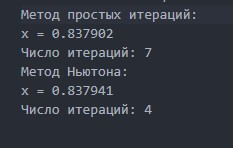
\includegraphics[width=.9\textwidth]{img1}
\end{figure}

\subsection{Исходный код}
\lstinputlisting{include/task_4_1.cpp}
\pagebreak

\section* {4.2. Решение краевой задачи для ОДУ 2-го порядка на указанном отрезке с помощью метода стрельбы и конечно-разностного метода}

\setcounter{subsection}{0}


\subsection{Постановка задачи}
Реализовать метод стрельбы и конечно-разностный метод решения краевой задачи для ОДУ в виде программ. С использованием разработанного программного обеспечения решить краевую задачу для обыкновенного дифференциального уравнения 2-го порядка на указанном отрезке. Оценить погрешность численного решения с использованием метода Рунге – Ромберга и путем сравнения с точным решением.  

{\bfseries Вариант:} 30 (был заменён, так как в 5 варианте неверно указано точное решение)
\begin{align*}
\text{Краевая задача: }
& (x^2 + 1) y'' - 2y = 0, \\
& y'(0) = 0,\\
& y(2) - y'(2) = 1 \\
\text{Точное решение: }
& y(x) = x^2 + 1 \\
\end{align*}
\pagebreak

\subsection{Результаты работы}
\begin{figure}[h!]
\centering
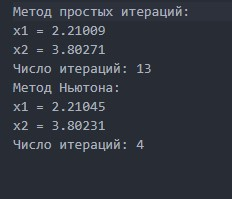
\includegraphics[width=.9\textwidth]{img2}
\end{figure}
\pagebreak

\subsection{Исходный код}
\lstinputlisting{include/task_4_2.cpp}
\pagebreak
